\begin{example}
    Let $p$ be a polynomial of degree $\le n$.
    Let $\varphi_i(x) = x^{i}$, i.e. $\varphi_0(x) = 1$, 
    $\varphi_1(x) = x$, and so on.
    \[
        x^2 + 2x + 3 = \varphi_2(x) + 2 \varphi_1(x) + 3 \varphi_0(x)
    \]
    Let $u_i = i + 1,\ i = 0, \dots, n$.
    Collocation matrix:
    \[
        \Phi = \begin{bmatrix}
            \varphi_0(u_0) & \dots & \varphi_n(u_0)\\
            \vdots & \ddots & \vdots\\
            \varphi_0(u_n) & \dots & \varphi_n(u_n)
        \end{bmatrix} = 
        \begin{bmatrix}
            1^0 & 1^1 & \dots & 1^n\\
            2^0 & 2^1 & \dots & 2^n\\
            \vdots & \vdots & \ddots & \vdots\\
            (n + 1)^0 & (n + 1)^1 & \dots & (n + 1)^n
        \end{bmatrix}
        \text{ --- Vandermonde matrix}
    \]
    As we can see, a Vandermonde matrix has very small entries (1)
    and very big ones ($(n + 1)^n$), therefore
    rounding errors can become relatively large even for small $n$.
    Therefore, $\varphi_i(x) = x^{i}$ is a bad choice of basis functions.

    Consider $n = 2$ and values $p_i$ as
    \[
        \begin{array}{c|c|c|c}
            u_i & 1 & 2 & 3\\
            \hline
            p_i & 2 & 5 & 10
        \end{array}
    \]
    Then
    \[
        \begin{bmatrix}
            1 & 1 & 1\\
            1 & 2 & 4\\
            1 & 3 & 9
        \end{bmatrix}
        \begin{pmatrix}
            \alpha_0 \\ \alpha_1 \\ \alpha_2
        \end{pmatrix} = \begin{pmatrix}
            -2 \\ 5 \\ 10
        \end{pmatrix}
    \]
    (basis functions at nodes $u_i \cdot \text{coefficients}$ = values)
    \begin{align*}
        \alpha_0 = 1,\ \alpha_1 = 0,\ \alpha_2 = 1 \implies
        p(u) &= 1 \cdot \varphi_0(u) + 0 \cdot \varphi_1(u) + 1 \cdot \varphi_2(u)
        \\&= 1 \cdot 1 + 0 \cdot u + 1 \cdot u^2
        \\&= 1 + u^2 \text{ --- the interpolating polynomial}
    \end{align*}
\end{example}

Can we find bases for polynomial spaces that leads to a more convenient collocation matrix?

\subsubsection{Lagrange interpolation}
Given $n + 1$ values/points
$p_1, \dots, p_n$ and corresponding nodes $u_0, \dots, u_n$
define the interpolating polynomial as
\[
    p(u) = \sum_{i = 0}^n p_i L_i^n(u) \quad \text{($n$ here is an upper index, not power)}
\]
where the so called Lagrange polynomial $L_i^n(n)$ of degree $n$
fullfills:
\[
    L_i^n(u_j) = \delta_{ij} = \begin{cases}
        1 & \text{if } i = j\\
        0 & \text{if } i \ne j
    \end{cases}
\]
(Such a function $\delta$ is called \text{Kronecker delta}.)
\newpage
\begin{example}
    \mbox{}
    \begin{itemize}
        \item {
            Lagrange polynomials of degree 2:
            \begin{center}   
                \begin{tikzpicture}
                    \begin{axis}[
                        axis x line=center,
                        axis y line=left,
                        axis line style={-{Stealth[scale=1.5]}},
                        xtick={0,1,2},
                        xticklabels={$u_0$, $u_1$, $u_2$},
                        ytick=\empty,
                        xmin=-1, xmax=3, ymin=-1, ymax=3,
                        unit vector ratio=1 1 1,
                        samples=100,
                    ]
                        \tikzset{graph/.style={very thick, smooth, domain=-1:3}}

                        \addplot[red, graph] {(x - 1) * (x - 2) / (-2)};
                        \addlegendentry{$L_0^2(u)$}

                        \addplot[green, graph] {(x - 0) * (x - 2) / (-1)};
                        \addlegendentry{$L_1^2(u)$}

                        \addplot[blue, graph] {(x - 0) * (x - 1) / 2};
                        \addlegendentry{$L_2^2(u)$}
                    \end{axis}
                \end{tikzpicture}
            \end{center}
        }
        \item {
            Degree 3:
            \begin{center}   
                \begin{tikzpicture}
                    \begin{axis}[
                        axis x line=center,
                        axis y line=left,
                        axis line style={-{Stealth[scale=1.5]}},
                        xtick={0,1,2,3},
                        xticklabels={$u_0$, $u_1$, $u_2$, $u_3$},
                        ytick=\empty,
                        xmin=-1, xmax=4, ymin=-1, ymax=2,
                        unit vector ratio=1 1 1,
                        samples=100,
                    ]
                        \tikzset{graph/.style={very thick, smooth, domain=-1:4}}
                        \addplot[blue, graph] {(x - 0) * (x - 1) * (x - 3) / (-2)};
                        \addlegendentry{$L_2^3(u)$}
                    \end{axis}
                \end{tikzpicture}
            \end{center}
        }
    \end{itemize}

    For $n=2$ these polynomials are defined as
    \begin{align*}
        &
        L_0^2(u) = \frac{(u - u_1)(u - u_2)}{(u_0 - u_1)(u_0 - u_2)}
        \\&
        L_1^2(u) = \frac{(u - u_0)(u - u_2)}{(u_1 - u_0)(u_1 - u_2)}
    \end{align*}
    The numerator makes sure that the polynomial is equal to zero at
    other nodes, and the denominator scales the whole polynomial
    so that it is equal to 1 at $u_1$.
\end{example}

In general, for $n \in \mathbb{N}$,
\[
    L_i^n(u) = \prod_{\substack{j=0 \\ j \ne i}}^n 
    \frac{(u - u_j)}{(u_i - u_j)}
\]
By construction, $L_i^n(u_j) = \delta_{ij}$.
\begin{example}
    \[ \begin{array}{c|c|c|c}
        u_i & 0 & 1 & 2\\
        \hline
        p_i & 2 & 4 & 3
    \end{array} \]
    \begin{enumerate}[font={\bfseries}, label={Step \arabic*.}]
        \item {
            Get Lagrange polynomial:
            \begin{align*}
                &
                L_0^2(u) =  \frac{(u - u_1)(u - u_2)}{(u_0 - u_1)(u_0 - u_2)} =
                \frac{(u - 1)(u - 2)}{(-1) \cdot (-2)} = \frac{1}{2} u^2 - \frac{3}{2}u + 1
                \\&
                L_1^2(u) = \dots = -u^2 + 2u
                \\&
                L_2^2(u) = \dots = \frac{1}{2} u^2 - \frac{1}{2} u
            \end{align*}
        }
        \item {
            Collocation matrix:
            \[
                \Phi = \begin{bmatrix}
                    L_0^2(u_0) & L_1^2(u_0) & L_2^2(u_0)\\
                    L_0^2(u_1) & L_1^2(u_1) & L_2^2(u_1)\\
                    L_0^2(u_2) & L_1^2(u_2) & L_2^2(u_2)
                \end{bmatrix} = \begin{bmatrix}
                    1 & 0 & 0\\
                    0 & 1 & 0\\
                    0 & 0 & 1\\
                \end{bmatrix} = I
            \]
        }
        \item {
            $\Phi \vec{\alpha} = \vec{p} \iff \vec{\alpha} = \vec{p}$
            so $p(u) = 2 L_0^2(u) + 4L_1^2(u) + 3L_2^2(u)$
        }
    \end{enumerate}
\end{example}
\begin{consequence}
    In Lagrange interpolation, the collocation matrix (by construction) is the identitiy matrix!
\end{consequence}

\textbf{Summary:}
\begin{itemize}
    \item {
        In Lagrange interpolation, basis functions are such that interpolation scheme becomes trivial.
    }
    \item {
        However, if one more node is added, the computations have to be redone.
    }
\end{itemize}

\subsubsection{Aitken's algorithm}
We want to evaluate $p(u)$ at one location $u^*$.
Then we can use Aitken's algorithm without directly computing $p(u)$.
\[
    L_i^n(u) = \prod_{\substack{j=0 \\ j \ne i}}^n 
    \frac{(u - u_j)}{(u_i - u_j)}
\]
The Lagrange polynomials have a so-called \textit{partition of unity} property:
\[
    \sum_{i=0}^n L_i^n(u) = 1
\]
(for proof use, e.g., $f(u) = 1$ as function that needs to be interpolated).

This allows for recursive definition of the Lagrange polynomials:

\begin{itemize}
    \item {
        For $n = 0$: $L_0^0(u) = 1$.
    }
    \item {
        For $n > 0$:
        \[
            L_i^n(u) = L_i^{n - 1}(u) \cdot \frac{u - u_n}{u_1 - u_n}
            \text{ for } i = 0, \dots, n - 1
        \]
        (The Lagrange polynomials from previous $n$ get one more root.)

        And
        \begin{align*}
            &
            L_n^n(u) \overset{\text{partition of unity}}{=} 1 - \sum_{i=0}^{n - 1} L_i^n(u) =
            1 - \sum_{i=0}^{n-1} L_i^{n-1}(u)\Bigl(\frac{u - u_n}{u_i - u_n}\Bigr)
            \overset{\text{partition of unity}}{=}
            \\&
            = \sum_{i=0}^{n-1} L_i^{n-1}(u)
            -\sum_{i=0}^{n-1} L_i^{n-1}(u) \cdot \Bigl(
                \frac{u - u_n}{u_i - u_n}
            \Bigr) =
            \sum_{i=0}^{n-1} L_i^{n-1}(u) 
            \Bigl(1 - \frac{u - u_n}{u_i - u_n}\Bigr)
        \end{align*}
        This recursive formula is basis for a simple algorithm to evaluate
        the Lagrange interpolating polynomials (Aitken's algorithm).
        \begin{align*}
            p(u) &= \sum_{i=0}^n p_i^0 L_i^n(u)
            \text{, where } p_i^0 = p_i \text{ --- given data}
            \\&= \sum_{i=0}^{n-1} p_i^0 L_i^n(u) + p_n^0 L_n^n(u)
            \\&= \sum_{i=0}^{n-1} p_i^0 L_{i}^{n-1}(u) \frac{u - u_n}{u_i - u_n} +
            p_n^0 \sum_{i=0}^{n-1} L_{i}^{n-1}(u) \Bigl(1 - \frac{u - u_n}{u_i - u_n}\Bigr)
            \text{ (from the recursive formula)}
            \\&= \sum_{i=0}^{n - 1} L_i^{n-1}(u) \biggl(
                p_i^0 \textcolor{red}{\frac{u - u_n}{u_i - u_n}} + p_n^0 \Bigl(
                    1 - \textcolor{red}{\frac{u - u_n}{u_i - u_n}}
                \Bigr)
            \biggr) =: p_i^1 \text{ for } i = 0, \dots, n - 1
            \\&= \sum_{i=0}^{n-1} p_i^1 L_i^{n-1}(u) = \dots
            = \sum_{i=0}^{n-2} p_i^2 L_i^{n-2}(u)
            \text{, where } p_i^2 \coloneqq
            p_i^1 \frac{u - u_{n-1}}{u_i - u_{n-1}} + p_{n-1}^1 \Bigl(
                    1 - \frac{u - u_{n-1}}{u_i - u_{n-1}}
            \Bigr)
            \\&= \dots = \sum_{i=0}^0 p_i^n L_i^0(u) = p_0^n
        \end{align*}
        and
        \[
            p_i^{k+1} = p_i^k \frac{u - u_{n-k}}{u_i - u_{n-k}} + p_{n-k}^k \Bigl(
            1 - \frac{u - u_{n-k}}{u_i - u_{n-k}}\Bigr)
        \]
        Evaluating $p_0^n$ for a fixed value of $n$ is equivalent
        to computing $p(u)$!
    }
\end{itemize}

\textbf{Scheme:}
\begin{center}
    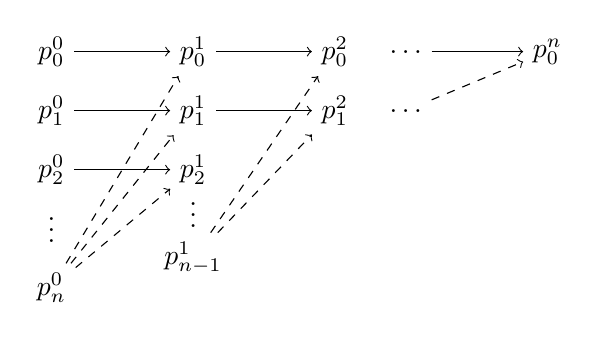
\begin{tikzpicture}[x=1.8cm,y=0.75cm]
        \node[] at (0, 0) (00) {$p_0^0$};
        \node[] at (0, -1) (01) {$p_1^0$};
        \node[] at (0, -2) (02) {$p_2^0$};
        \node[] at (0, -2.875) {$\vdots$};
        \node[] at (0, -4) (0n) {$p_n^0$};

        
        \node[] at (1, 0) (10) {$p_0^1$};
        \node[] at (1, -1) (11) {$p_1^1$};
        \node[] at (1, -2) (12) {$p_2^1$};
        \node[] at (1, -2.625) {$\vdots$};
        \node[] at (1, -3.5) (1n1) {$p_{n-1}^1$};

        \node[] at (2, 0) (20) {$p_0^2$};
        \node[] at (2, -1) (21) {$p_1^2$};

        \node[] at (2.5, 0) (30) {$\dots$};
        \node[] at (2.5, -1) (31) {$\dots$};

        \node[] at (3.5, 0) (40) {$p_0^n$};

        \draw [->] (00) -- (10);
        \draw [->] (01) -- (11);
        \draw [->] (02) -- (12);
        \draw [->] (10) -- (20);
        \draw [->] (11) -- (21);
        \draw [->] (30) -- (40);
        \draw [dashed,->] (31) -- (40);
        \draw [dashed,->] (0n) -- (10);
        \draw [dashed,->] (0n) -- (11);
        \draw [dashed,->] (0n) -- (12);
        \draw [dashed,->] (1n1) -- (20);
        \draw [dashed,->] (1n1) -- (21);
    \end{tikzpicture}
\end{center}
where $\longrightarrow$ means:
\[ {} \cdot \frac{u - u_{n-k}}{u_i - u_{n-k}} \]
and $\dashrightarrow$ means:
\[ {} \cdot \Bigl(1 - \frac{u - u_{n-k}}{u_i - u_{n-k}}\Bigr) \]

\begin{example}
    \[ \begin{array}{c|c|c|c}
        u_i & 0 & 1 & 2\\
        \hline
        p_i & 2 & 4 & 3
    \end{array} \]
    We want to compute $p(1 / 2)$. $n = 2$.
    For $k=0$ we have
    $p_0^0 = 2,\ p_1^0 = 4,\ p_2^0 = 3$. We need to calculate the coefficients to get
    from $p_i^0$ to $p_i^1$:
    \begin{align*}
        \text{for } i = 0:\
        \frac{u - u_2}{u_0 - u_2} = \frac{\frac{1}{2} - 2}{0 - 2} = \textcolor{red}{\frac{3}{4}}
        \qquad&
        1 - \frac{3}{4} = \textcolor{blue}{\frac{1}{4}}
        \\
        \text{ for } i = 1:\
        \frac{u - u_2}{u_1 - u_2} = \frac{\frac{1}{2} - 2}{1 - 2} = \textcolor{red}{\frac{3}{2}}
        \qquad&
        1 - \frac{3}{2} = \textcolor{blue}{-\frac{1}{2}}
    \end{align*}
    Now compute $p_i^1$:
    \begin{center}
        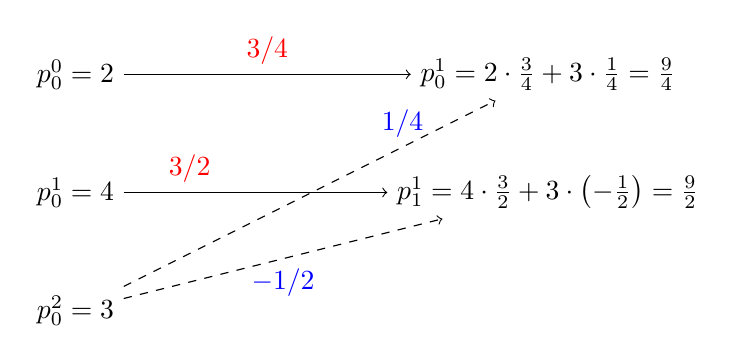
\begin{tikzpicture}[x=6cm,y=1.5cm]
            \node[] at (0, 0) (00) {$p_0^0 = 2$};
            \node[] at (0, -1) (01) {$p_0^1 = 4$};
            \node[] at (0, -2) (02) {$p_0^2 = 3$};

            \node at (1, 0) (10) {$p_0^1 = 2 \cdot \frac{3}{4} + 3 \cdot \frac{1}{4} = \frac{9}{4}$};
            \node at (1, -1) (11) {$p_1^1 = 4 \cdot \frac{3}{2} + 3 \cdot \bigl(-\frac{1}{2}\bigr) = \frac{9}{2}$};
    
            \draw [->] (00) -- node [above,midway] {$\textcolor{red}{3/4}$} (10);
            \draw [->] (01) -- node [above,near start] {$\textcolor{red}{3/2}$} (11);
            \draw [dashed,->] (02) -- node [above,near end] {$\textcolor{blue}{1/4}$} (10);
            \draw [dashed,->] (02) -- node [below,midway] {$\textcolor{blue}{-1/2}$} (11);
        \end{tikzpicture}
    \end{center}
    For $k=1$, we have
    $p_0^1 = \frac{9}{4},\ p_1^1 = \frac{9}{2}$.
    For $i = 0$:
    \[
        \frac{u - u_1}{u_0 - u_1} = \frac{\frac{1}{2} - 1}{0 - 1} = \textcolor{red}{\frac{1}{2}}
        \qquad
        1 - \frac{1}{2} = \textcolor{blue}{\frac{1}{2}}
    \]
    Now compute $p_0^2$:
    \begin{center}
        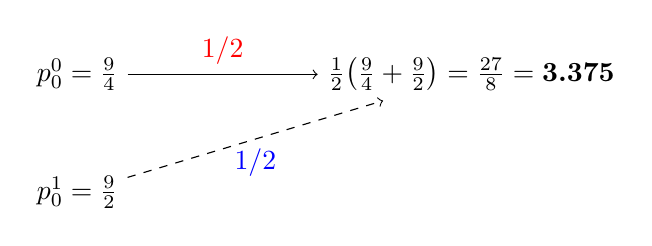
\begin{tikzpicture}[x=5cm,y=1.5cm]
            \node[] at (0, 0) (00) {$p_0^0 = \frac{9}{4}$};
            \node[] at (0, -1) (01) {$p_0^1 = \frac{9}{2}$};

            \node at (1, 0) (10) {$\frac{1}{2}\bigl(\frac{9}{4} + \frac{9}{2}\bigr) = \frac{27}{8} = \textbf{3.375}$};
    
            \draw [->] (00) -- node [above,midway] {$\textcolor{red}{1/2}$} (10);
            \draw [dashed,->] (01) -- node [below,below] {$\textcolor{blue}{1/2}$} (10);
        \end{tikzpicture}
    \end{center}
\end{example}

\textbf{Summary:} Aitken's algorithm is an iterative process
for evaluating Lagrange interpolation polynomials without actually constructing
them. It has a complexity of $\mathcal{O}(n^2)$, but it needs
just half of the steps that are needed by explicit construction of $p(n)$.